\documentclass{beamer}
\usetheme{CambridgeUS}
%kod alternativne verzije koristim
%\usetheme{MoreblueLight}

\usepackage[croatian]{babel}
\usepackage[utf8]{inputenc}
\usepackage[T1]{fontenc}
\usepackage[autostyle]{csquotes}
\usepackage{amsmath}
\usepackage{url}
\usepackage{fancybox}
\usepackage{wasysym}
\usepackage{listings}
\usepackage{verbatim}
\usepackage{multirow}
\usepackage{graphicx}
\usepackage{algorithm2e}
\usepackage[style=alphabetic]{biblatex}

\newcommand{\A}[1]{#1&\texttt{\string#1}\hspace*{1ex}}


\hypersetup{plainpages=false,bookmarksopen,linkcolor=violet,%
pdfpagemode=FullScreen,colorlinks=true%
}
\hypersetup{pdftitle={Prezentacije}}
\hypersetup{baseurl={http://www.math.hr}}
\hypersetup{pdfsubject={LaTeX}}
\hypersetup{pdfauthor={Ivica Nakić}}

\lstset{language=[LaTeX]TeX,extendedchars=true,backgroundcolor=\color{gray!20},identifierstyle=,stringstyle=\rmfamily,%
columns=flexible,showstringspaces=false,keywordstyle=\color{violet}\bfseries}

\lstset{literate=%
{Š}{{\v{S}}}1
{Đ}{{\Dj{}}}1
{Č}{{\v{C}}}1
{Ć}{{\'C}}1
{Ž}{{\v{Z}}}1
{š}{{\v{s}}}1
{đ}{{\dj{}}}1
{č}{{\v{c}}}1
{ć}{{\'c}}1
{ž}{{\v{z}}}1
}

\newtheorem{thm}{Teorem}
\newtheorem*{rol}{Rolleov teorem}
\newtheorem{cor}[thm]{Korolar}
\theoremstyle{remark}
\newtheorem{slutnja}{Slutnja}
\newtheorem{ex}{Primjer}
\theoremstyle{definition}
\newtheorem{dfn}[slutnja]{Definicija}

\addbibresource{P2.bib}

\title{\LaTeX{} --- Prezentacije i ostalo}
\subtitle{}
\author{Ivica Nakić \\ \texttt{nakic@math.hr}}
\institute[PMF--MO]{Matematički odsjek Prirodoslovno--matematičkog fakulteta}
\date[2015/16]{Matematički software, 2015/16}


\begin{document}

\begin{frame}
  \maketitle  
\end{frame}

\begin{frame}
\frametitle{Pregled}
  \tableofcontents  
\end{frame}

\section{Plutajući objekti}

\begin{frame}[fragile]
\frametitle{Plutajući objekti}
Pri unosu većih nedjeljivih objekata, kao što su npr. tablice ili slike, često je teško odrediti pravo mjesto u tekstu gdje ih treba smjestiti e da bi prijelom teksta bio odgovarajući.

Stoga brigu o tome možemo prepustiti \LaTeX{}u uz pomoć \emph{plutajućih} okolina za slike i tablice. 

Ukoliko npr. okolinu \textcolor{violet}{tabular} stavimo unutar okoline \textcolor{violet}{table}, ta tablica će biti stavljena u dokument tako da minimizira praznine na stranicama.

\LaTeX{}u možemo sugerirati gdje preferiramo da se tablica pojavi pomoću opcionalnih parametara. Sintaksa je:
\begin{lstlisting}
\begin{table}[parametri]
...
\end{table}
\end{lstlisting}
\end{frame}

\begin{frame}
\frametitle{Plutajući objekti 2}
Parametri:
\begin{description}
\item[\textcolor{brown}{H}] ako je moguće, staviti tablicu na mjesto gdje smo je unijeli
\item[\textcolor{brown}{h}] ako je moguće, staviti tablicu (otprilike) na mjesto gdje smo je unijeli
\item[\textcolor{brown}{t}] ako je moguće, staviti tablicu na vrh stranice
\item[\textcolor{brown}{b}] ako je moguće, staviti tablicu na dno stranice
\item[\textcolor{brown}{p}] staviti tablicu na stranicu na kojoj se nalaze samo plutajući objekti.
\end{description}
Možemo staviti jedan ili više parametara. Predefinirane opcije su \textcolor{brown}{tbp}.

Sintaksa okoline \textcolor{violet}{figure} za unos plutajućih slika je ista. 

Ali kako se unose slike u \LaTeX u?

Za to nam služi paket \textcolor{violet}{graphicx}. 
\end{frame}

\section{Slike}

\begin{frame}[fragile]
\frametitle{Slike}
Najjednostavnije sintaksa je \textcolor{violet}{\textbackslash includegraphics\{ime\_slike\}}. Pri generiranju PDFa dozvoljeni formati su 
\textcolor{brown}{jpg}, \textcolor{brown}{png}, \textcolor{brown}{pdf} i \textcolor{brown}{tiff} (u zaglavlje stavimo 
\textcolor{violet}{\textbackslash usepackage[pdftex]\{graphicx\}}. 

Dodatne opcije naredbe  \textcolor{violet}{\textbackslash includegraphics} nam omogućavaju niz transformacija slike, Npr. 
\begin{lstlisting}
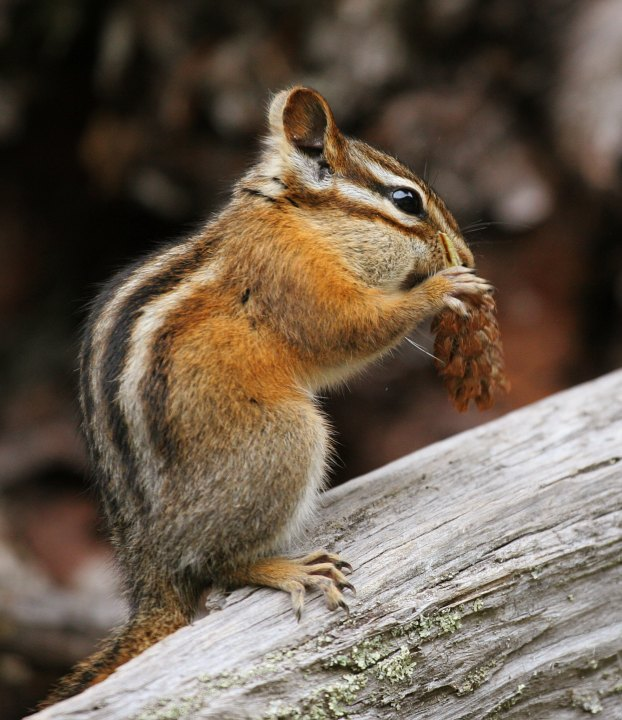
\includegraphics[width=2cm,angle=45]{Tamias_minimus.jpg}
\end{lstlisting}
\begin{figure}
\centering
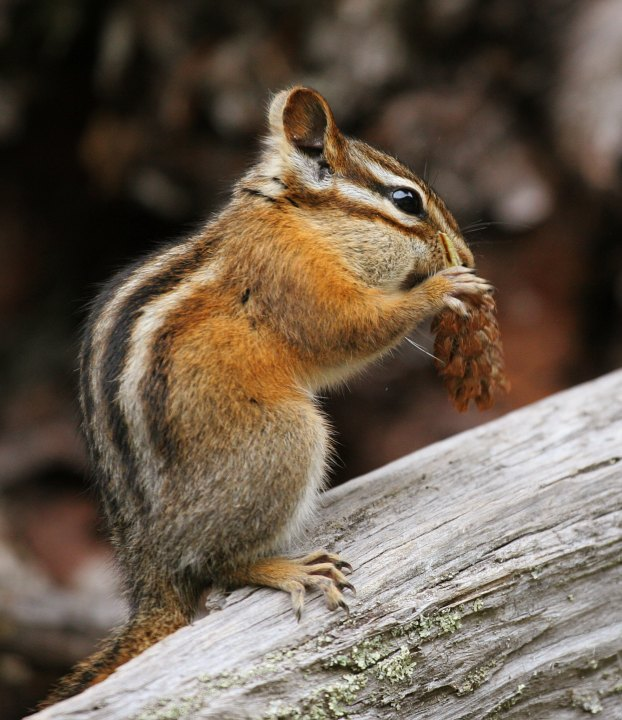
\includegraphics[width=2cm,angle=45]{Tamias_minimus.jpg}
\caption{Chipmunk (Tamias minimus), vrsta vjeverice}
\end{figure}
\end{frame}

\begin{frame}
\frametitle{Slike 2}
Tekst ispod slike je dobijen pomoću naredbe \textcolor{violet}{\textbackslash caption}. Ona se koristi samo kod plutajućih objekata.
\pause

\begin{minipage}{6cm}
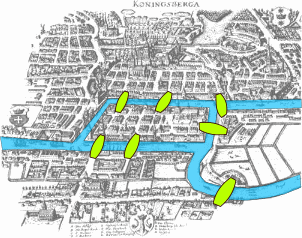
\includegraphics[angle=180,scale=0.5]{Konigsberg_bridges.png}
\end{minipage}
\begin{minipage}[c]{5cm}
Ovu sliku smo npr.\ smanjili i rotirali: \textcolor{violet}{\textbackslash includegraphics [angle=180,scale=0.5] \{Konigsberg\_bridges.png\}}. I nismo
koristili naredbu \textcolor{violet}{\textbackslash caption}.	
\end{minipage}
\end{frame}

\begin{frame}
\frametitle{Još o \textcolor{violet}{graphicx} paketu}
Paket \textcolor{violet}{graphicx} sadrži i druge naredbe. Npr\textcolor{violet}{\textbackslash scalebox}: 

\textcolor{brown}{
\scalebox{3}[2]{Zdravo!}
} 

je dobijeno pomoću k\^oda \textcolor{violet}{\textbackslash scalebox\{3\}[2]\{Zdravo!\}}, a 

\textcolor{brown}{
\scalebox{-1}[1]{Zdravo!}
} 

pomoću k\^oda \textcolor{violet}{\textbackslash scalebox\{-1\}[1]\{Zdravo!\}}.
\end{frame}

\section{Projekti}

\begin{frame}[fragile]
\frametitle{Veći dokumenti}
Ukoliko pišemo veći dokument, poželjno je tekst smjestiti u više datoteka, npr. svako poglavlje u zasebnu datoteku. 

Tekst iz drugih datoteka uključujemo pomoću naredbi \textcolor{violet}{\textbackslash input}, \textcolor{violet}{\textbackslash include} i \textcolor{violet}{\textbackslash includeonly}. Npr.\ 
\begin{lstlisting}
\documentclasss[12pt]{report}
\includeonly{pogl2.tex,pogl3.tex}
%--zaglavlje--------
\begin{document}
\include{pogl1.tex}
\include{pogl2.tex}
\include{pogl3.tex}
\end{document}
\end{lstlisting}

Datoteke \textcolor{brown}{pogl1.tex}, \textcolor{brown}{pogl2.tex} i \textcolor{brown}{pogl3.tex} se ne tretiraju kao zasebni \LaTeX{} dokumenti te u njima nema zaglavlja, već krećemo od npr. \textcolor{brown}{\textbackslash chapter\{...\}}.
\end{frame}

\section{Bibliografija}

\begin{frame}[fragile]
\frametitle{Bibliografija}
Bibliografiju možemo unositi direktno u \LaTeX{} datoteku ili je možemo spremiti u zasebnu datoteku. Mi ćemo obraditi drugi način, koji pruža puno veću fleksibilnost.

Najprije kreiramo bibliografsku bazu koja se sastoji od bibliografskih jedinica oblika
\begin{lstlisting}
@book {knuth1,
    AUTHOR = {Knuth, Donald E.},
     TITLE = {Digital typography},
    SERIES = {CSLI Lecture Notes},
    VOLUME = {78},
 PUBLISHER = {CSLI Publications},
   ADDRESS = {Stanford, CA},
      YEAR = {1999},
     PAGES = {xvi+685},
}
\end{lstlisting}
\end{frame}

\begin{frame}[fragile]
\frametitle{Bibliografija 2}
Tipovi bibliografskih jedinica su \textcolor{violet}{@book}, \textcolor{violet}{@article}, \textcolor{violet}{@manual}, \textcolor{violet}{@proceedings},...

Obično se bibliografska baza ne kreira ručno, nego se skida s Interneta ili izvozi iz aplikacija. Npr.\ podatke za matematičke knjige i članke u tzv.\ 
\textit{bibtex} formatu možemo naći na stranici \href{http://www.ams.org/mathscinet/search}{http://www.ams.org/mathscinet/search}, a i mnogi stručni pretraživači (npr.\ \href{http://scholar.google.com/}{Google Scholar}) te razne aplikacije nude izvoz podataka u \textit{bibtex} formatu.

Da bi smo bibliografiju uključili u naš dokument, na mjestu u tekstu gdje želimo imati popis literature stavimo 
\textcolor{violet}{\textbackslash printbibliography}, a negdje u zaglavlje stavimo:

\begin{lstlisting}
\usepackage[style=alphabetic]{biblatex}
\addbibresource{ime_datoteke}
\end{lstlisting}

Ovdje je \textcolor{violet}{alphabetic} jedan od mnogih stilova koje nam nudi biblatex.

\textcolor{violet}{ime\_datoteke} je ime datoteke u kojoj su smješteni bibliografski podaci (i koja obavezno ima {sufiks} \textcolor{brown}{.bib}).
\end{frame}

\begin{frame}[fragile]
\frametitle{Bibliografija 3}
Kako bi u tekstu citirali Knuthovu knjigu, trebamo samo na odgovarajuće mjesto staviti \textcolor{violet}{\textbackslash cite\{knuth1\}}, kao npr.\ ovdje \cite{knuth1}.

U popisu literature će se nalaziti samo citirani radovi. Ukoliko želimo da se u popisu literature pojavi i neka necitirana referenca, dovoljno je bilo gdje u tekst ubaciti npr. \textcolor{violet}{\textbackslash nocite\{van2012\}}. Ukoliko pak želimo uključiti sve podatke iz bibliografske baze, trebamo negdje u dokument staviti  
\textcolor{violet}{\textbackslash nocite\{*\}}.
\nocite{*}

Kako procesiramo dokument koji ima  bibliografiju? Najprije procesiramo \LaTeX{} datoteku, potom procesiramo \textit{bibtex} datoteku (pomoću programa 
\textcolor{brown}{biber}), te potom još dvaput procesiramo \LaTeX{} datoteku. Obično editori koji podržavaju \LaTeX{} format sami brinu o ovoj proceduri.

U Sagemath oblaku za \textcolor{brown}{Build} naredbu treba staviti
\begin{lstlisting}
latexmk -pdf -f -latex="pdflatex -interact=nonstopmode %S" file.tex
\end{lstlisting}

\end{frame}

\begin{frame}
\frametitle{Popis literature}
\printbibliography
\end{frame}

\section{Interaktivnost}

\begin{frame}
\frametitle{\textcolor{brown}{\textbackslash hyperref}}
Pomoću \LaTeX a možemo kreirati i interaktivne dokumente. Npr. unutar PDF dokumenta kreiranog \LaTeX om možemo stavljati interaktivne elemente kao što su linkovi, forme itd. 

Tu funkcionalnost omogućava paket \textcolor{violet}{hyperref}. Npr.\ ukoliko želimo staviti link na \TeX{} user group stranicu, jednostavno upišemo
\textcolor{violet}{\textbackslash href\{http://www.tug.org\}\{\textbackslash LARGE TUG\}}.

Uključivanjem paketa \textcolor{violet}{hyperref} automatski sve reference u dokumentu postaju i linkovi. Naravno, i unutar samog teksta možemo postavljati sidra (\textit{anchors}) i linkove pomoću naredbi
 \textcolor{violet}{\textbackslash hypertarget\{ime\_sidra\}\{tekst\}} i  \textcolor{violet}{\textbackslash hyperlink\{ime\_sidra\}\{tekst\}}. 
\end{frame}

\section{Ispis k\^odova i algoritama}

\begin{frame}
\frametitle{Algoritmi}

Postoji jako puno paketa koji služe za ispis programskih k\^odova, a jedan od popularnijih je \textcolor{brown}{algorithm2e}. 

\begin{algorithm}[H]
\KwIn{
Integers  $a \geq 0$ and $b\geq 0$}	
\KwOut{\textsc{GCD} of $a$ and $b$}
\While{$b \neq 0$} {
$r \leftarrow a \bmod b$\;
$a \leftarrow b$\;
$b \leftarrow r$\;	
}
\caption{Euclidean algorithm}
\end{algorithm}
\end{frame}

\begin{frame}[fragile]
\frametitle{Algoritmi}
K\^od za prethodni slajd je:
\begin{lstlisting}
\begin{algorithm}[H]
\KwIn{
Integers  $a \geq 0$ and $b\geq 0$}	
\KwOut{\textsc{GCD} of $a$ and $b$}
\While{$b \neq 0$} {
$r \leftarrow a \bmod b$\;
$a \leftarrow b$\;
$b \leftarrow r$\;	
}
\caption{Euclidean algorithm}
\end{algorithm}	
\end{lstlisting}
\end{frame}

\begin{frame}[fragile]
\frametitle{Ispisivanje programskih k\^odova}
U ovim prezentacijama korišten je paket \textcolor{brown}{listings}, u kojem je predefiniran ogroman broj programskih jezika, kao i HTML, \LaTeX{} itd.
Jedan primjer upotrebe za k\^od pisan u Javi: 
\begin{lstlisting}[language=Java
,firstline=2
,lastline=4
,caption=Hello World.
,label=example]
public class Greetings {
	public static void main( String[] args ) {
		System.out.println( "Hello world!" );
	}
}
\end{lstlisting}  
\end{frame}

\begin{frame}[fragile]
\frametitle{Paket \textcolor{brown}{listings}}
K\^od za prethodni slajd:
\begin{verbatim}
\begin{lstlisting}[language=Java
,firstline=2
,lastline=4
,caption=Hello World.
,label=example]
public class Greetings {
	public static void main( String[] args ) {
		System.out.println( "Hello world!" );
	}
}
\end{lstlisting}     	
\end{verbatim}    
\end{frame}

\begin{frame}[fragile]
\frametitle{Predefinirane vrijednosti}
Pomoću naredbe \textcolor{violet}{\textbackslash lstset} mogu se postaviti predefinirane vrijednosti za okolinu 
\textcolor{violet}{\textbackslash lstlisting}. Naprimjer, u zaglavlju dokumenata za ove prezentacije se koristi ova naredba na sljedeći način:
\begin{lstlisting}
\lstset{
language=[LaTeX]TeX,extendedchars=true,
backgroundcolor=\color{gray!20},
identifierstyle=,stringstyle=\rmfamily,
columns=flexible,showstringspaces=false,
keywordstyle=\color{violet}\bfseries}	
\end{lstlisting}
\end{frame}

\section{Prezentacije}

\begin{frame}
\frametitle{Pravljenje prezentacija u \LaTeX u}
Za pravljenje prezentacija uobičajeno je koristiti paket \textcolor{violet}{beamer}. 

Uključivanje beamera: \textcolor{violet}{\textbackslash documentclass\{beamer\}}.


\end{frame}

\begin{frame}[fragile]
  \frametitle{Moj novi slajd}
  \framesubtitle{moj podnaslov} 
 Svaki slajd se piše unutar okoline \textcolor{violet}{frame}.  
  \begin{columns}
  \column{3cm}
  \begin{itemize}
    \item Prvi
    \item Drugi
  \end{itemize}
 \column{6cm}
\begin{lstlisting}
  \frametitle{Moj novi slajd}
  \framesubtitle{moj podnaslov}  
  \begin{columns}
  \column{5cm}
  \begin{itemize}
    \item Prvi
    \item Drugi
  \end{itemize}	
\end{lstlisting}
\end{columns}
\end{frame}


\begin{frame}
  \frametitle{Primjer 2}
  \framesubtitle{Podnaslov} 
  \begin{itemize}
    \only<1->{\item Prva formula $\sin^2 x+\cos^2 x=1$}
    \uncover<2->{\item Druga formula $e^{i\pi}=-1$}
    \uncover<3>{\item Treća formula \[ \sum_{i=1}^n i=\frac{n(n+1)}{2}\]}
    \only<1->{\item Četvrta formula $\alpha \trianglerighteq \beta \gtrapprox \gamma$}
  \end{itemize}
\end{frame}

\begin{frame}[fragile]
\frametitle{K\^od za prethodni slajd}
\begin{lstlisting}
  \begin{itemize}
    \only<1->{\item Prva formula ...}
    \uncover<2->{\item Druga formula ...}
    \uncover<3>{\item Treća formula ...}
    \only<1->{\item Četvrta formula ...}
  \end{itemize}		
\end{lstlisting}
\end{frame}

\begin{frame}
  \frametitle{Zašto Beamer?}
  \begin{itemize}[<+->]
  \item Zato što se piše u  \LaTeX{}u.
  \item Izlazni format je PDF.
  \item Lako se mijenja izgled prezentacije.
  \item Već napisani tekst se može lako iskoristiti za prezentaciju.
  \end{itemize}
\end{frame}

\begin{frame}[fragile]
\frametitle{K\^od za prethodni slajd}
\begin{lstlisting}
  \begin{itemize}[<+->]
  \item Zato što se piše u  \LaTeX{}u.
  \item Izlazni format je PDF.
  \item Lako se mijenja izgled prezentacije.
  \item Već napisani tekst se može lako iskoristiti za prezentaciju.
  \end{itemize}    	
\end{lstlisting}    
\end{frame}

\begin{frame}
  \frametitle{Što su prosti brojevi?}
  \framesubtitle{Slajd posuđen iz \cite{beamerUserGuide}}
  \begin{dfn}
     \alert{Prosti broj} je broj koji ima točno dva djelitelja.
  \end{dfn}
  \pause
  \begin{ex}
    \begin{itemize}[<+->]
    \item 2 je prost (djelitelji su  1 i 2).
    \item 3 je prost (djelitelji su  1 i 3).
    \item 4 nije prost (\alert{tri} djelitelja: 1, 2, i 4).
    \end{itemize}
  \end{ex}
\end{frame}

\begin{frame}[fragile]
\frametitle{K\^od za prethodni slajd}
\begin{lstlisting}
  \begin{dfn}
     \alert{Prosti broj} je broj koji ima točno dva djelitelja.
  \end{dfn}
  \pause
  \begin{ex}
    \begin{itemize}[<+->]
    \item 2 je prost (djelitelji su  1 i 2).
    \item 3 je prost (djelitelji su  1 i 3).
    \item 4 nije prost (\alert{tri} djelitelja: 1, 2, i 4).
    \end{itemize}
  \end{ex}  	
\end{lstlisting}    
\end{frame}

\begin{frame}
  \frametitle{Ne postoji najveći prosti broj}
  \framesubtitle{Slajd posuđen iz \cite{beamerUserGuide}}
  \begin{thm}
    Ne postoji najveći prosti broj.
  \end{thm}
  \begin{proof}
    \begin{enumerate}
    \item<1-> Pretpostavimo da je $p$ najveći prosti broj.
    \item<2-> Neka je $q$ umnožak prvih $p$ brojeva.
    \item<3-> Tada $q + 1$ nije djeljiv ni s jednim od njih.
    \item<1-> Dakle, $q + 1$ je također prost i veći je od $p$.\qedhere
    \end{enumerate}
  \end{proof}
  \uncover<4->{Dokaz je koristio postupak \emph{reductio ad absurdum}.}
\end{frame}

\begin{frame}[fragile]
\frametitle{K\^od za prethodni slajd}
\begin{lstlisting}
  \begin{thm}
    Ne postoji najveći prosti broj.
  \end{thm}
  \begin{proof}
    \begin{enumerate}
    \item<1-> Pretpostavimo da je $p$ najveći prosti broj.
    \item<2-> Neka je $q$ umnožak prvih $p$ brojeva.
    \item<3-> Tada $q + 1$ nije djeljiv ni s jednim od njih.
    \item<1-> Dakle, $q + 1$ je također prost i veći je od $p$.\qedhere
    \end{enumerate}
  \end{proof}   
\end{lstlisting}    
\end{frame}

\begin{frame}
  \frametitle{Dva stupca}
  \framesubtitle{Svaki je stupac centriran}
  \begin{columns}
    \column{.5\textwidth}
          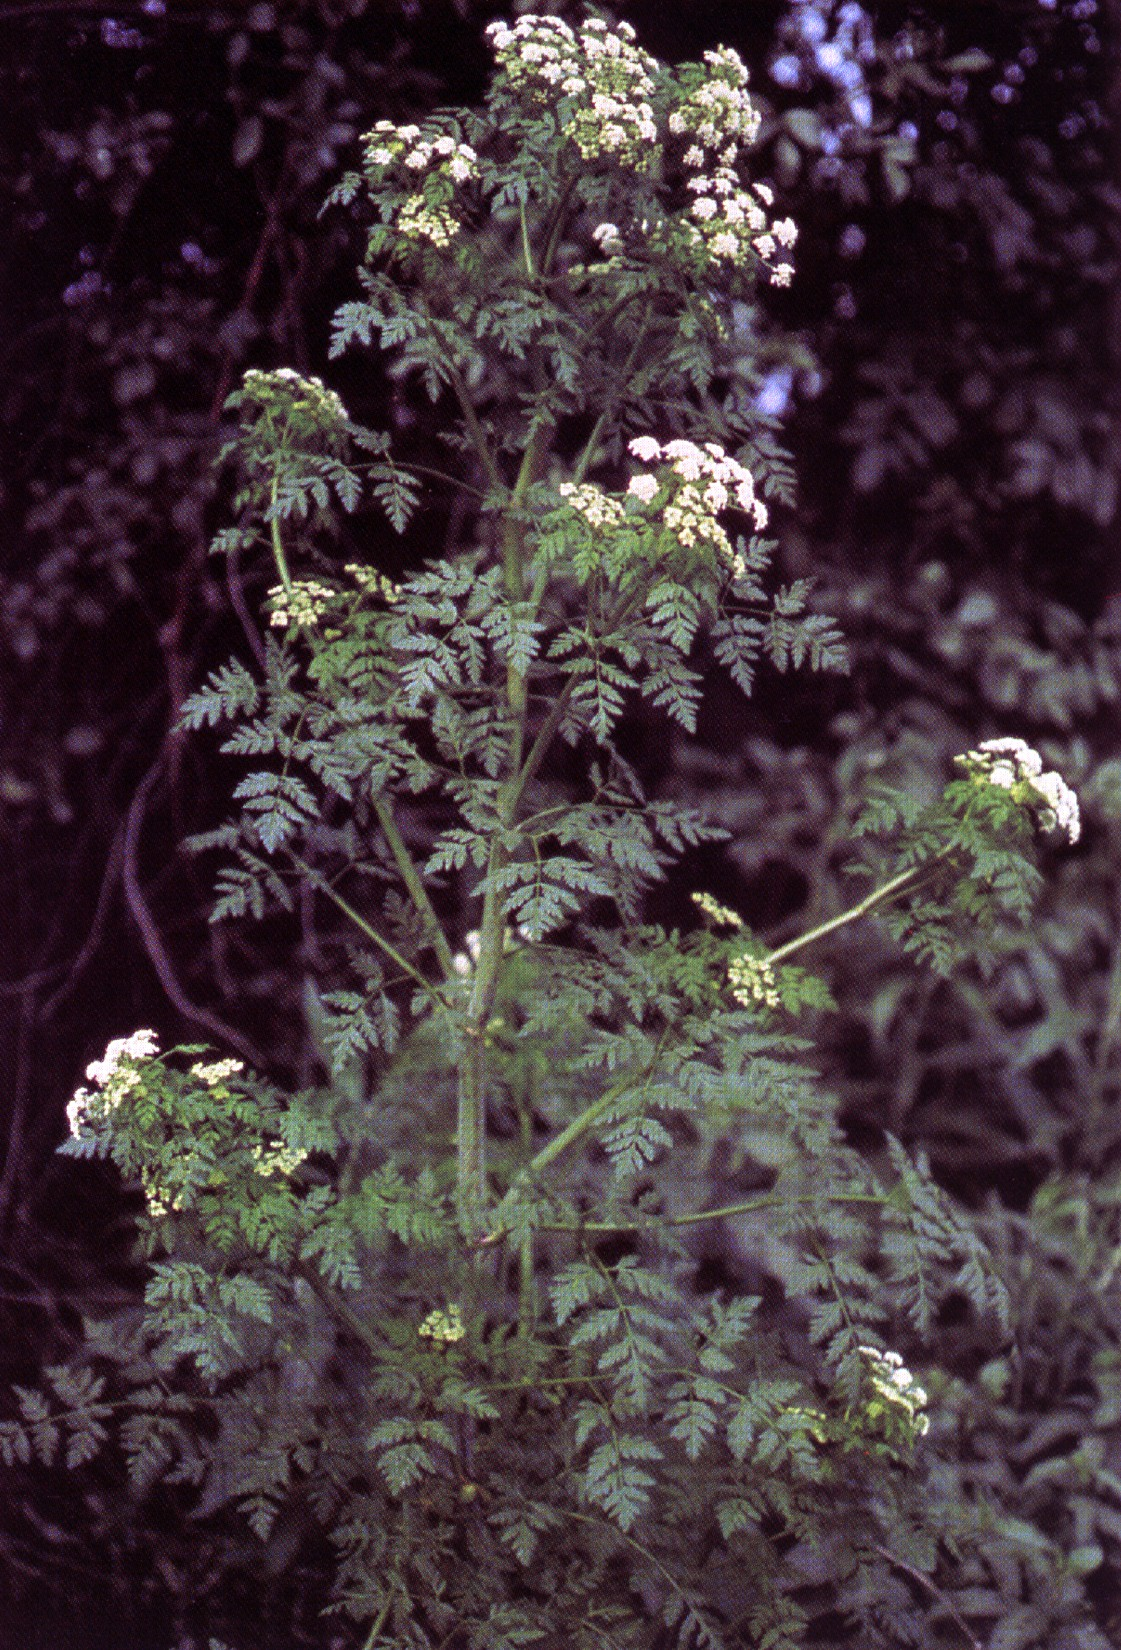
\includegraphics[height=0.8\textheight]{Conium.jpg}%
    \column{.5\textwidth}
    \begin{itemize}[<+->]
    \item Točka 1
    \item Točka 2
    \end{itemize}
    \onslide<3->{ 
    \begin{block}{Još jedna kutija}
      Lorem ipsum dolor sit amet, consectetuer adipiscing elit
    \end{block}
    }
  \end{columns}
\transdissolve<3>
\end{frame}

\begin{frame}[fragile]
\frametitle{K\^od za prethodni slajd}
\begin{lstlisting}
  \begin{columns}
    \column{.5\textwidth}
          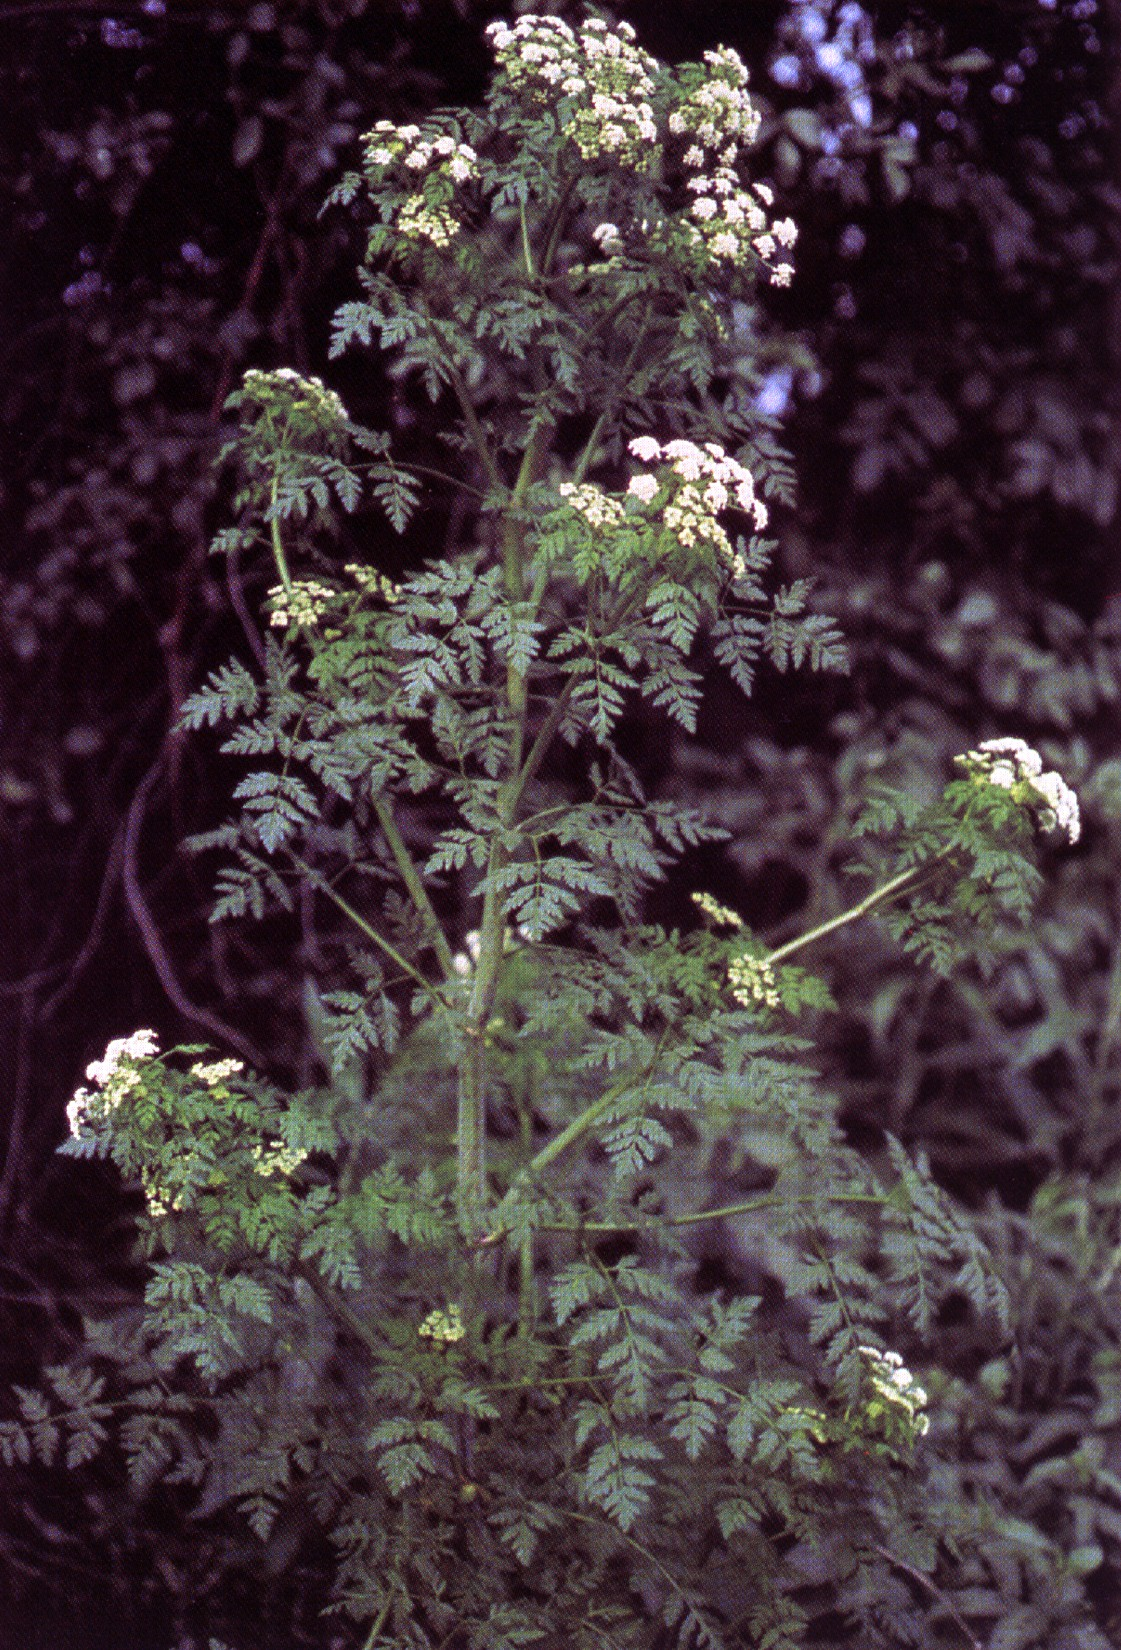
\includegraphics[height=0.8\textheight]{Conium.jpg}%
    \column{.5\textwidth}
    \begin{itemize}[<+->]
    \item Točka 1
    \item Točka 2
    \end{itemize}
    \onslide<3->{ 
    \begin{block}{Još jedna kutija}
      Lorem ipsum dolor sit amet, consectetuer adipiscing elit
    \end{block}
    }
  \end{columns}
\transdissolve<3>
\end{columns}
\end{lstlisting}    
\end{frame}

\begin{frame}
  \frametitle{Dva stupca}
  \framesubtitle{Vrhovi stupaca su centrirani}
  \begin{columns}[t]
    \column{.5\textwidth}
     \begin{block}{Kutija}
        Lorem ipsum dolor sit amet, consectetuer adipiscing elit
      \end{block}
    \column{.5\textwidth}
      \begin{block}{Kutija}
           Lorem ipsum dolor sit amet, consectetuer adipiscing elit, sed diam nonummy nibh euismod tincidunt ut laoreet dolore magna aliquam erat volutpat. Ut wisi enim ad minim veniam, quis nostrud exerci tation ullamcorper suscipit lobortis nisl ut aliquip ex ea commodo consequat. 
      \end{block}
  \end{columns}
  \pause

  Vrhovi stupaca su centrirani zbog opcije \textcolor{violet}{[t]} -- format je \textcolor{violet}{\textbackslash begin\{columns\}[t]}.
\end{frame}

\begin{frame}
  Predefinirano je da je tekst u slajdu vertikalno centriran. 
\end{frame}


\begin{frame}[t]
  Ali ovaj nije ... razlog je opet opcija \textcolor{violet}{[t]} -- sada uz okolinu \textcolor{violet}{frame}:
  \textcolor{violet}{\textbackslash begin\{frame\}[t]}.
\end{frame}


\begin{frame}[plain]
  Trebate \alert{cijeli slajd} i ništa manje od toga? 

  Ovdje se radi o opciji \textcolor{violet}{[plain]} -- opet uz okolinu \textcolor{violet}{frame}.
\end{frame}

\begin{frame}[fragile]
  \frametitle{Ostalo}
Ukoliko se unutar slajda koriste okoline ili naredbe za prikazivanje manipulaciju tekstom (kao \textcolor{violet}{lstlisting} ili slično) okolina \textcolor{violet}{frame} treba imati opciju \textcolor{violet}{fragile}:
\begin{lstlisting}
\begin{frame}[fragile]   
 \end{lstlisting}
 ili se može definirati nova okolina koja tu opciju ima automatski uključenu:
 \begin{lstlisting}
\newenvironment{myframe}[0] 
  {\begin{frame}[fragile]}
  {\end{frame}}    
  \end{lstlisting} 
Beamer ima jako puno predefiniranih tema (stilova izgleda) koji se zovu po gradovima. Ova prezentacija koristi temu CambridgeUS. Sintaksa je 
\begin{lstlisting}
\usetheme{CambridgeUS}    
\end{lstlisting}  
\end{frame}

\section{Za kraj}

\begin{frame}
\transwipe[direction=90,duration=3]
\frametitle{Ostali paketi i klase koje vrijedi spomenuti}
{\Huge \textbf{Paketi}: biblatex, booktabs, cleveref, cool, coverpage, enumerate, fancyhdr, geometry, mathdesign, mathtools, microtype, nag, nicefrac, prettyref, siunitx, todonotes}

\bigskip

{\Huge \textbf{Klase}: KOMA, memoir}    
\end{frame}

\begin{frame}
\frametitle{Zadatak za vježbu}
    
Kreirajte prezentaciju koja sadrži dva plutajuća objekta, bibliografiju, linkove unutrašnje i vanjske te neki k\^od.

\end{frame}
\end{document}